\documentclass[11pt]{article}

\usepackage[margin=1in]{geometry}
\usepackage[T1]{fontenc}
\usepackage{ifxetex,ifluatex}
\ifnum 0\ifxetex 1\fi\ifluatex 1\fi=0 % if pdftex
  \usepackage[utf8]{inputenc}
\fi
\usepackage{lmodern}
\usepackage{microtype}

\usepackage{amsmath,amssymb,amsthm,mathtools}
\usepackage{stmaryrd}
\usepackage{tikz}
\usetikzlibrary{arrows.meta,shapes.misc,positioning,calc,decorations.pathreplacing}
\usepackage{tikz-cd}
\usepackage{hyperref}
\usepackage[nameinlink,capitalise]{cleveref}
\usepackage{enumitem}

\usepackage{titlesec}

\newcommand{\sectionbreak}{\clearpage}

% ==========================================
%  Category macros
% ==========================================
\newcommand{\cat}[1]{\mathbf{#1}}
\newcommand{\OGraph}{\cat{OGraph}}
\newcommand{\Graph}{\cat{Graph}}
\newcommand{\Hyp}{\cat{Hyp}}
\newcommand{\Set}{\cat{Set}}

% ==========================================
%  AION / RMG Names
% ==========================================
\newcommand{\RMG}{\mathrm{RMG}}
\newcommand{\Hist}{\mathrm{Hist}}

% Inline project names (math-safe)
\newcommand{\AION}{\text{AI}\textOmega\text{N}}
\newcommand{\COMPUTER}{\text{C}\textOmega\text{MPUTER}}
\newcommand{\AIONWordmarkSerif}{\textrm{AION}}
\newcommand{\AIONInline}{\textrm{AION}}
\newcommand{\AIONSignature}[1][1]{\AIONWordmarkSerif}
\newcommand{\AIONProjectURL}{\url{https://flyingrobots.dev}}
\newcommand{\FULL}{\textbf{FULL}}
\newcommand{\ZK}{\textbf{ZK}}
\newcommand{\OPAQUE}{\textbf{OPAQUE}}

% ==========================================
%  Rewrite / Footprint helpers
% ==========================================
% We use \rightsquigarrow to denote rewrite steps.
\newcommand{\Rewrite}{\rightsquigarrow}
\newcommand{\To}{\rightarrow}
\newcommand{\mono}{\hookrightarrow}

\newcommand{\Del}{\mathrm{Del}}
\newcommand{\Use}{\mathrm{Use}}
\newcommand{\Foot}{\mathrm{Foot}}
\newcommand{\RMGState}{\mathrm{RMGState}}
\newcommand{\Recon}{\mathrm{Recon}}
\newcommand{\Apply}{\mathrm{Apply}}
\newcommand{\Trans}{\mathrm{Trans}}

% ==========================================
%  Theorem environments
% ==========================================
\theoremstyle{plain}
\newtheorem{theorem}{Theorem}[section]
\newtheorem{lemma}[theorem]{Lemma}
\newtheorem{proposition}[theorem]{Proposition}
\newtheorem{corollary}[theorem]{Corollary}

\theoremstyle{definition}
\newtheorem{definition}[theorem]{Definition}
\newtheorem{example}[theorem]{Example}
\newtheorem{remark}[theorem]{Remark}

% ==========================================
% ==========================================
%  Wordmark: Display + Inline (uses serif roman + Greek Omega)
% ==========================================
\renewcommand{\AIONWordmarkSerif}{%
  {\rmfamily\Large A\kern0.15em I\kern0.2em \ensuremath{\Omega}\kern0.1em N}%
}

\renewcommand{\AIONInline}{%
  {\rmfamily A\kern0.12em I\kern0.16em \ensuremath{\Omega}\kern0.1em N}%
}

% ---------------------------------------------------------
% AION LOGO (circle + diamond + square)
% Numeric values tuned for the current wordmark size; see comments below.
% ---------------------------------------------------------
\pgfkeys{/aionlogo/.cd,
  scale/.store in=\aionlogoScale, scale=1,
  radius/.store in=\aionlogoRadius, radius=1.05,
  square/.store in=\aionlogoSquare, square=0.55,
  outerwidth/.store in=\aionlogoOuterWidth, outerwidth=0.52pt,
  innerwidth/.store in=\aionlogoInnerWidth, innerwidth=0.32pt
}

\newcommand{\AIONLogo}[1][1]{%
  \pgfkeys{/aionlogo,scale=#1}%
  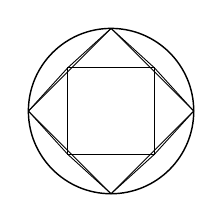
\begin{tikzpicture}[
      scale=\aionlogoScale,
      baseline=-0.55ex,% aligns with the wordmark baseline
      line cap=round,
      line join=round]
    \pgfmathsetmacro{\R}{\aionlogoRadius}
    \pgfmathsetmacro{\s}{\aionlogoSquare}
    \path (0,\R) coordinate (N)
          (0,-\R) coordinate (S)
          (\R,0) coordinate (E)
          (-\R,0) coordinate (W)
          (\s,\s) coordinate (NE)
          (-\s,\s) coordinate (NW)
          (\s,-\s) coordinate (SE)
          (-\s,-\s) coordinate (SW);

    \draw[line width=\aionlogoOuterWidth] (0,0) circle (\R);
    \draw[line width=\aionlogoInnerWidth] (N) -- (E) -- (S) -- (W) -- cycle;
    \draw[line width=\aionlogoInnerWidth] (NW) rectangle (SE);
    \draw[line width=\aionlogoInnerWidth] (N) -- (NE);
    \draw[line width=\aionlogoInnerWidth] (N) -- (NW);
    \draw[line width=\aionlogoInnerWidth] (S) -- (SE);
    \draw[line width=\aionlogoInnerWidth] (S) -- (SW);
    \draw[line width=\aionlogoInnerWidth] (E) -- (NE);
    \draw[line width=\aionlogoInnerWidth] (E) -- (SE);
    \draw[line width=\aionlogoInnerWidth] (W) -- (NW);
    \draw[line width=\aionlogoInnerWidth] (W) -- (SW);
    % Node dots intentionally omitted to keep the emblem minimal.
  \end{tikzpicture}%
}

\renewcommand{\AIONSignature}[1][0.28]{%
  % Raise/kerning values tuned for optical alignment with the wordmark.
  \raisebox{0.02em}{\smash{\AIONLogo[#1]}}\kern0.65em{\AIONWordmarkSerif}%
}


\title{Computational Holography\\[0.4em]
  \large Recursive Metagraphs, Rulial Distance,\\
  and the Foundations for Deterministic Multiway Computation}

\author{James Ross\\
  \small Independent Researcher\\
  \small \texttt{james@flyingrobots.dev}}

\date{November 2025}

\begin{document}

\maketitle

\begin{abstract}
We develop a formal model of \emph{computational holography}: a way of
representing a computation so that its entire interior evolution is
encoded on the ``boundary''---the provenance payload on a single
recursive metagraph edge.  Building on double--pushout graph rewriting
in adhesive categories, we define Recursive Metagraphs (RMGs), give a
deterministic concurrent operational semantics, prove tick-level
confluence and a two-plane commutation theorem, and state conditions for
global confluence.  We then introduce provenance payloads and show how
they provide an information-complete, holographic encoding of a
computation's history.  Finally, we define an MDL-based \emph{rulial
distance} between observers, relate RMG dynamics to multiway systems and
the Ruliad, and outline how this structure underlies the \AION{}
\COMPUTER{}---a new, provenance-native machine model with deterministic,
confluent tick semantics and a quasi-pseudometric geometry on
observers.
\end{abstract}

\tableofcontents

\sectionbreak
\section{Introduction}
\label{sec:intro}

Modern computation is built on mutable state and loosely specified
concurrency.  As systems become distributed, multi-core, and
AI-mediated, this leads to nondeterminism, opaque failure modes,
unreproducible behavior, and fundamentally incomplete provenance.

The goal of this work is to develop a mathematically precise alternative
model in which:

\begin{itemize}[leftmargin=*]
  \item global state is represented as a recursively nested,
    graph-shaped object;
  \item all evolution of that state is given by well-typed graph
    rewrites;
  \item under an explicit independence discipline and
    no-delete/no-clone-under-descent invariants, the operational
    semantics is deterministic (up to typed open graph isomorphism)
    and confluent at the level of ``ticks'' of computation
    (\cref{thm:tick-confluence,thm:two-plane,thm:global}); and
  \item the \emph{entire} interior evolution of a computation is stored
    in a compact \emph{provenance payload} attached to a single edge,
    providing an information-complete ``holographic'' encoding.
\end{itemize}

The technical starting point is algebraic graph transformation using the
double--pushout (DPO) approach in adhesive categories, together with the
Recursive Metagraph (RMG) object model we define in Section~\ref{sec:rmg}.
We extend this setting with:

\begin{enumerate}[leftmargin=*]
  \item a precise notion of RMG state and its category;
  \item a two-plane concurrent operational semantics with
    attachment--then--skeleton publication, together with
    confluence results: tick-level determinism and two-plane
    commutation (Theorems~\ref{thm:tick-confluence} and
    \ref{thm:two-plane}), and, under standard rewrite-theory
    hypotheses, global confluence (Theorem~\ref{thm:global});
  \item a provenance payload calculus giving \emph{computational
    holography};
  \item an MDL-based quasi-pseudometric on observers, the \emph{rulial
    distance}, and a correspondence between RMG derivations and
    multiway systems that clarifies the relationship to Wolfram's
    Ruliad.
\end{enumerate}

We deliberately keep the system-level \AION{} stack\footnote{%
Pronounced ``eye-ON'' (rhymes with \emph{aeon}), with stress on the second syllable.}
(AIONOS, Echo, Wesley, etc.) mostly offstage in this paper, mentioning
it only to motivate the mathematics.  The companion ``\COMPUTER{}''
paper will build on these results to define the full machine model and
operating system.

\medskip
\noindent
\textbf{Key contributions.}
The main results of this paper are:
\begin{enumerate}[leftmargin=5mm]
  \item \emph{Tick-level confluence} (Theorem~\ref{thm:tick-confluence}):
    parallel independent RMG rewrites commute, yielding per-tick
    deterministic semantics independent of scheduler serialization
    order;
  \item \emph{Two-plane commutation} (Theorem~\ref{thm:two-plane}):
    attachment and skeleton updates can be applied in either order up to
    isomorphism, via a fibration structure;
  \item \emph{Worldline uniqueness} (Corollary~\ref{cor:worldline-uniqueness}):
    global uniqueness of complete derivation worldlines up to typed
    open graph isomorphism, extending per-tick commutation to
    scheduler-independent whole runs;
  \item \emph{Computational holography} (Theorem~\ref{thm:holography}):
    the boundary data $(S_0,P)$ is information-complete with respect to
    the interior evolution, enabling reconstruction of the full
    derivation volume;
  \item \emph{Rulial distance} (Theorem~\ref{thm:rulial-triangle}):
    an MDL-based quasi-pseudometric on observers that quantifies the
    complexity of translating between different views of the same
    computation.
\end{enumerate}

\input{sections/rmg}
\sectionbreak
\section{DPO Rewriting on Recursive Metagraphs}
\label{sec:dpo-rmg}

We recall double--pushout with interfaces (DPOI) rewriting on typed open
graphs and lift it to RMG states.

\subsection{Typed open graphs and DPOI rules}

Let $T$ be a finite set of types.
Let $\OGraph_T$ be the category of $T$-typed open graphs, whose objects
are cospans of monomorphisms $I \hookrightarrow G \hookleftarrow O$ and
whose morphisms are commuting maps of cospans.  This category is
adhesive; in particular,
pushouts along monos exist and form Van Kampen squares.

\begin{definition}[DPOI rule]
A \emph{DPOI rule} is a span of monos in $\OGraph_T$
\[
  p = (L \xleftarrow{\ell} K \xrightarrow{r} R)
\]
with $L$ the left-hand side, $K$ the interface, and $R$ the right-hand
side.  A \emph{match} of $p$ in a host graph $G$ is a mono
$m : L \mono G$ satisfying the usual gluing conditions: the
dangling condition and the identification condition.
\end{definition}

Given a match, the DPO construction yields a rewrite step
$G \Rewrite_p H$ by computing a pushout complement and a pushout:

\[
\begin{tikzcd}
  K \arrow[r,"\ell"] \arrow[d,"k"'] &
  L \arrow[d,"m"] \\
  D \arrow[r] & G
\end{tikzcd}
\qquad
\begin{tikzcd}
  K \arrow[r,"r"] \arrow[d,"k"'] &
  R \arrow[d] \\
  D \arrow[r] & H
\end{tikzcd}
\]

All arrows are monos in $\OGraph_T$.

\subsection{RMG states as two-plane objects}

We work with RMG states and tick semantics as defined in
\cref{def:rmg-state,def:rmg-tick}.  For convenience, recall that an
RMG state consists of a typed open-graph skeleton together with
attachment fibres, and a tick applies a scheduler-admissible batch of
attachment and skeleton DPOI steps subject to the independence and
no-delete/no-clone-under-descent conditions introduced in
\cref{sec:determinism}.

We now turn to the determinism properties of this semantics.

\sectionbreak
\section{Determinism and Confluence}
\label{sec:determinism}

We sketch the concurrency discipline, define independence, and state the
main confluence theorems for tick-level execution.

\subsection{Scheduler state and footprints}

The global runtime state includes, in addition to the current RMG state,
a multiset of \emph{pending rewrites} with matches, footprints, and
phases.  Operationally this is described in the AION engine
specification. For the mathematics, we abstract it
as follows.

\begin{definition}[Footprint]
Given a rule $p$ and match $m : L \mono G$, define the \emph{delete set}
and \emph{use set} as
\[
  \Del(m) = m(L \setminus K), \qquad
  \Use(m) = m(L).
\]
A \emph{footprint} $F(m)$ records these sets, together with read/write
sets for attachments and a factor mask used to enforce additional
ordering constraints.
\end{definition}

\begin{definition}[Independence]
Two matches $m_1,m_2$ are (parallel) \emph{independent} if
\[
  \Del(m_1) \cap \Use(m_2) = \emptyset, \qquad
  \Del(m_2) \cap \Use(m_1) = \emptyset,
\]
and both matches satisfy the gluing conditions.  A scheduler-admissible
batch is a finite family of matches that are pairwise independent in
this sense and respect the attachment invariants.
\end{definition}

\subsection{Tick semantics and scheduler confluence}

We recall the basic setting.  Work in the adhesive category
$\OGraph_T$ of typed open graphs.  A DPOI rule is a span of monos
$p = (L \xleftarrow{\ell} K \xrightarrow{r} R)$; a match is a mono
$m : L \hookrightarrow G$ satisfying the usual gluing conditions
(dangling and identification).  A DPOI step $G \Rightarrow_p H$ is
given by the standard double square (pushout complement + pushout).

\begin{definition}[RMG state and tick]
An RMG state is a triple
\[
  \mathcal{U} \;=\; (G; \alpha, \beta)
\]
with skeleton $G \in \OGraph_T$ and attachment objects
$\alpha(v), \beta(e) \in \OGraph_T$ in the fibers over each
node $v \in V(G)$ and edge $e \in E(G)$.

A \emph{tick} consists of:
\begin{itemize}[leftmargin=*]
  \item a finite family $A$ of attachment DPOI steps in the fibers
    $\alpha(v), \beta(e)$;
  \item a finite family $S = \{(p_i,m_i)\}_{i\in I}$ of skeleton DPOI
    steps on $G$ such that the matches $\{m_i\}$ are pairwise parallel
    independent.
\end{itemize}
The tick obeys the \emph{no-delete-under-descent} invariant: if some
attachment step in $A$ touches $\alpha(v)$ or $\beta(e)$, then no
concurrent skeleton step in $S$ may delete $v$ or $e$.
Operationally, a tick publishes attachments first and then skeleton.
\end{definition}

The scheduler computes a maximal independent set of matches in the
sense above, using a safe over-approximation of $\Use\cup\Del$; we do
not repeat the implementation details here.

\begin{theorem}[Tick-level confluence]\label{thm:tick-confluence}
Let $\mathcal{U}$ be an RMG state and let
$A, S=\{(p_i,m_i)\}_{i\in I}$ form a tick as in the definition above.
Let $\sigma$ range over permutations of $I$.  For each $\sigma$, form
the serial composite
\[
   \mathcal{U}
      \;\Rewrite^{A}\;
   \mathcal{U}^{(0)}_\sigma
      \;\Rewrite^{(p_{\sigma(1)},m_{\sigma(1)})}\;
   \mathcal{U}^{(1)}_\sigma
      \;\Rewrite^{(p_{\sigma(2)},m_{\sigma(2)})}\;
   \cdots
      \;\Rewrite^{(p_{\sigma(|I|)},m_{\sigma(|I|)})}\;
   \mathcal{U}^{(|I|)}_\sigma.
\]
Then all results $\mathcal{U}^{(|I|)}_\sigma$ are isomorphic as RMG
states.  In particular, the effect of the tick is deterministic up to
typed open-graph isomorphism, independent of the serialisation order
chosen by the scheduler.
\end{theorem}

\begin{proof}
We separate the argument into the skeleton part and the attachment
part.

\emph{Skeleton.}
Consider only the skeleton matches $\{m_i : L_i \hookrightarrow G\}$.
By hypothesis, these matches are pairwise parallel independent.  By
the Concurrency / Parallel Independence Theorem for DPO rewriting in
adhesive categories (see, e.g.,~\cite{EEPT06}), parallel independent
steps commute: for any $i \neq j$ we have a diagram
\[
  G \;\Rightarrow_{(p_i,m_i)}\; G_i \;\Rightarrow_{(p_j,m'_j)}\; G_{ij}
  \quad\text{and}\quad
  G \;\Rightarrow_{(p_j,m_j)}\; G_j \;\Rightarrow_{(p_i,m'_i)}\; G_{ji}
\]
where both two-step derivations exist and the results $G_{ij}$ and
$G_{ji}$ are isomorphic.  The rewritten matches $m'_i, m'_j$ are
obtained by the standard reindexing construction of the concurrency
theorem.

We now induct on $|I|$ to obtain order-independence for the entire
family.

For $|I| = 0$ or $1$ the claim is trivial.  For $|I| = 2$ it is exactly
the commuting-square case of the concurrency theorem.

Assume the property holds for all scheduler-admissible families of
size $k$.  Let $S$ have size $k+1$.  Pick any index $j \in I$ and
factor an arbitrary serial order as
\[
  G \Rewrite^{(p_{i_1},m_{i_1})} \cdots
    \Rewrite^{(p_{i_k},m_{i_k})} G'
    \Rewrite^{(p_j,m'_j)} G''.
\]
By the induction hypothesis, the prefix of length $k$ yields a result
unique up to isomorphism, regardless of the order of the $k$ steps.
Now compare any two permutations of the full $(k+1)$ steps.  One can
be obtained from the other by a finite sequence of adjacent swaps.
Each adjacent swap exchanges two parallel independent steps; by the
two-step concurrency theorem, the corresponding length-$(k+1)$
derivations commute up to isomorphism.  Thus, by finite induction on
the number of swaps, all serialisations of the skeleton batch produce
isomorphic skeletons.

\emph{Attachments.}
Attachment steps live in the product of fibers
$\prod_{x\in V(G)\cup E(G)} \OGraph_T$, one fiber per node or edge.
Within a fixed tick, attachment steps are DPOI steps in these fibers
that do not change the skeleton $G$ itself.  Because the fibers form a
product category, DPOI steps in distinct fibers are trivially parallel
independent and commute strictly.

By the no-delete-under-descent invariant, any position $x$ whose
attachment $\alpha(x)$ or $\beta(x)$ is touched in this tick must lie
in the preserved interface $K_i$ of every concurrent skeleton step
$(p_i,m_i)$; in particular, skeleton rewriting does not delete $x$.
Skeleton steps are DPO pushouts along monos and therefore induce
reindexing isomorphisms on the fibers over preserved positions.
Hence, attachment updates may be taken to occur in a fixed copy of
each fiber and then transported along these isomorphisms without
affecting the result.

\emph{Putting the planes together.}
By definition of a tick, we always apply attachments before skeleton.
From the previous paragraph, the attachments part is independent of
the serialisation order of the skeleton part; and from the skeleton
argument, the skeleton result is independent (up to iso) of the
serialisation order of $S$.  Therefore the composite effect of the
tick is unique up to RMG isomorphism, independent of the order in
which the scheduler executes the individual steps.
\end{proof}

\subsection{Two-plane commutation via a fibration}

We now justify the two-plane discipline more structurally, using a
simple fibration view.

Let $\RMGState$ be the category of RMG states and RMG morphisms
(skeleton morphisms together with compatible fiber morphisms).  There
is a forgetful functor
\[
  \pi : \RMGState \;\longrightarrow\; \OGraph_T
\]
sending $(G;\alpha,\beta)$ to its skeleton $G$ and acting on morphisms
componentwise.  This functor is a (Grothendieck) fibration whose
fibers are products of copies of $\OGraph_T$:
\[
  \pi^{-1}(G) \;\cong\; \prod_{x\in V(G)\cup E(G)} \OGraph_T.
\]
In particular, given a mono $u : G \hookrightarrow G'$ in the base,
there is a reindexing functor
\[
  u^\ast : \pi^{-1}(G') \longrightarrow \pi^{-1}(G)
\]
which transports attachments along $u$ by precomposition.

An \emph{attachment step} is a DPOI step in some fiber
$\pi^{-1}(G)$; a \emph{skeleton step} is a DPOI step in the base
$\OGraph_T$.  Both are built from pushouts along monos.

\begin{theorem}[Two-plane commutation]\label{thm:two-plane}
Let $\mathcal{U} = (G;\alpha,\beta)$ be an RMG state.  Let
$A : \mathcal{U} \Rewrite \mathcal{U}_A$ be a finite composite of
attachment steps in the fiber over $G$, and let
$S : G \Rewrite G'$ be a composite of skeleton DPOI steps such that
no step in $S$ deletes or clones any position whose attachment is
touched by $A$ (no-delete/no-clone under descent).  Then there exists
an attachment composite $A' : (G';\alpha',\beta') \Rightarrow
(G';\alpha'',\beta'')$ in the fiber over $G'$ such that the following
square in $\RMGState$ commutes up to isomorphism:
\[
\begin{tikzcd}
  (G;\alpha,\beta) \arrow[r,"A"] \arrow[d,"S"']
    & (G;\alpha_A,\beta_A) \arrow[d,"S'"] \\
  (G';\alpha',\beta') \arrow[r,"A'"']
    & (G';\alpha'',\beta'')
\end{tikzcd}
\]
In particular, applying attachments then skeleton yields the same
result (up to iso) as applying skeleton then the transported
attachments.
\end{theorem}

\begin{figure}[t]
  \centering
  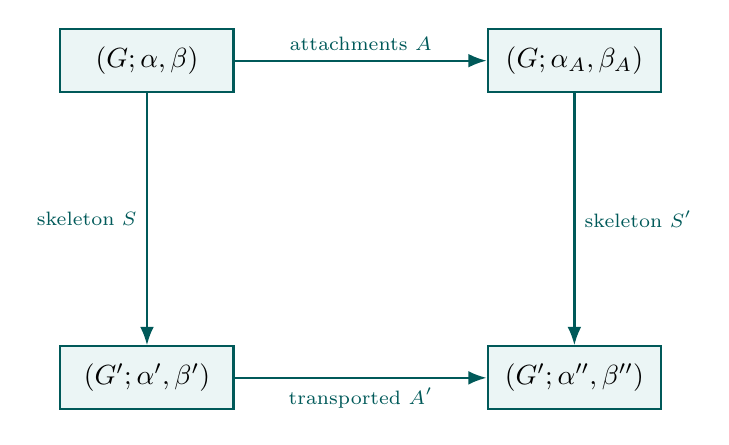
\begin{tikzpicture}[
      node distance=32mm,
      obj/.style={rectangle,draw=teal!70!black,fill=teal!8,thick,minimum width=22mm,
                  minimum height=8mm,align=center},
      arr/.style={-Latex,thick,teal!70!black},
      >=Latex
    ]

    \node[obj] (U)   {$(G;\alpha,\beta)$};
    \node[obj,right=of U] (UA)  {$(G;\alpha_A,\beta_A)$};
    \node[obj,below=of U] (US)  {$(G';\alpha',\beta')$};
    \node[obj,below=of UA] (USA) {$(G';\alpha'',\beta'')$};

    \draw[arr] (U)  -- node[above]{\scriptsize attachments $A$} (UA);
    \draw[arr] (U)  -- node[left]{\scriptsize skeleton $S$} (US);
    \draw[arr] (UA) -- node[right]{\scriptsize skeleton $S'$} (USA);
    \draw[arr] (US) -- node[below]{\scriptsize transported $A'$} (USA);

  \end{tikzpicture}
  \caption{Two-plane commutation: attachment updates $A$ in the fiber over $G$ commute with skeleton rewriting $S$ in the base, up to transporting the attachment steps along the skeleton morphism. Theorem~\ref{thm:two-plane} shows that the two paths in the square yield isomorphic RMG states.}
  \label{fig:two-plane-square}
\end{figure}

\begin{proof}
Write the skeleton composite $S$ as a sequence of DPOI steps
\[
  G = G_0 \Rewrite G_1 \Rewrite \cdots \Rewrite G_n = G'.
\]
Each step $G_{k-1} \Rewrite G_k$ is a pushout along a mono in
$\OGraph_T$.  Because $\OGraph_T$ is adhesive, pushouts along monos
are Van Kampen squares and stable under pullback~\cite{LS06}.

\smallskip
\noindent
The no-delete/no-clone-under-descent hypothesis ensures that every
position $x$ whose attachment is touched by $A$ lies in the preserved
interface of each skeleton step.  Thus, along the composite mono
$u : G \hookrightarrow G'$, the reindexing functor
$u^\ast : \pi^{-1}(G') \to \pi^{-1}(G)$ is an isomorphism on the
fibers corresponding to positions touched by $A$; informally, the
skeleton only renames those attachment slots.

\smallskip
\noindent
Consider first a single attachment step in the fiber over some
position $x$:
\[
  (G;\alpha,\beta) \Rightarrow_A (G;\alpha_A,\beta_A),
\]
given by a DPOI double square in the corresponding component of the
fiber $\pi^{-1}(G) \cong \prod_x \OGraph_T$.  Forming the pullback of
this square along the mono $u : G \hookrightarrow G'$ yields a square
in the fiber over $G'$; by stability of pushout complements and
Van Kampen, this square is again a DPOI step, which we denote by
$A'$:
\[
  (G';\alpha',\beta') \Rightarrow_{A'} (G';\alpha'',\beta'').
\]
At the level of the total category $\RMGState$ we thus obtain a
commuting cube whose back face is the original attachment step, whose
bottom face is the skeleton step, and whose front face is the
transported attachment step.  All vertical faces are pullbacks and all
horizontal faces are pushouts along monos; Van Kampen ensures that the
top and bottom composites are isomorphic.

\smallskip
\noindent
Iterating this construction over the finite families of attachment and
skeleton steps yields a composite cube whose front and back faces are
the two composites $S\circ A$ and $A'\circ S'$ in the statement.  By
pasting of Van Kampen squares, the induced morphism between the top
and bottom objects is an isomorphism in $\RMGState$.  Hence the
diagram commutes up to isomorphism.
\end{proof}

\subsection{Global confluence}

To obtain global Church--Rosser properties for the entire rewrite
system, additional hypotheses are required.  We invoke the standard
critical-pair lemma and Newman's lemma for terminating systems:

\begin{theorem}[Conditional global confluence]\label{thm:global}
Let $R$ be a finite DPOI rule set.  Suppose that:
\begin{enumerate}[leftmargin=*]
  \item every DPOI critical pair of $R$ is joinable (modulo boundary
    isomorphism), and
  \item the induced rewrite relation is terminating on the class of
    states considered, or admits a decreasing-diagrams labelling.
\end{enumerate}
Then the rewrite relation is confluent.
\end{theorem}

This theorem applies directly to the skeleton plane; together with the
attachment invariants and two-plane commutation, it yields uniqueness of
\emph{worldlines} at the level of RMG states when the rule pack
satisfies these conditions.

The upshot is that, under explicit and checkable rule-pack assumptions,
the runtime has a unique deterministic evolution from any given initial
state.  This is the key precondition for holographic provenance: there
is exactly one interior history to encode.
\input{sections/holography}
\input{sections/wormholes}
\sectionbreak
\section{Rulial Distance: A Computable Metric on Observer Space}
\label{sec:rulial}

We next formalize observers and an MDL-based distance between them, the
\emph{rulial distance}.  This provides a geometry on different
descriptions of the same underlying RMG universe.

\subsection{Observers as functors}

Fix an RMG universe $(U,R)$ and its history category
$\Hist(U,R)$ whose objects are states and whose morphisms are derivation
paths between them.  An \emph{observer} is a functor
\[
  O : \Hist(U,R) \To \mathcal{Y},
\]
where $\mathcal{Y}$ is a suitable category of observations (symbol
streams, trace graphs, etc.), subject to resource budgets on time and
memory.

Different observers may:

\begin{itemize}[leftmargin=*]
  \item choose different projections of the same wormhole payloads;
  \item aggregate or forget structure;
  \item expose different notions of causality.
\end{itemize}

\subsection{Translators and MDL cost}

A \emph{translator} between observers $O_1$ and $O_2$ is a functorial
construction $T : O_1 \Rewrite O_2$ realized as a small DPOI
transducer, together with a distortion metric on outputs.

\paragraph{Example (SQL$\leftrightarrow$AST translator).}
Consider two observers of an RMG universe modeling a database
query planner.  Observer $O_1$ sees the wormhole payload $P$ as
a sequence of AST transformations (parse tree $\to$ optimized AST
$\to$ query plan), while observer $O_2$ sees only the initial SQL
string and final execution trace.  A translator $T_{12}$ must
reconstruct the SQL from the AST evolution: it can parse the initial
AST root, emit the corresponding SQL, and summarize the execution
steps by their side effects.  The reverse translator $T_{21}$ parses
the SQL and heuristically infers an AST evolution consistent with the
execution trace, incurring some distortion.  The description lengths
$\mathrm{DL}(T_{12}), \mathrm{DL}(T_{21})$ and distortion costs
quantify how ``close'' these two viewpoints are in rulial space.

Let $\mathrm{DL}(T)$ be a prefix-code description length for $T$
(MDL cost), and let $\mathrm{Dist}$ be a distortion metric on observed
traces.  Intuitively, we measure how far two observers are by asking:
how complex is a program that translates the traces of $O_1$ into those
of $O_2$ (and back again), and how much distortion does that translation
incur?  Minimum Description Length (MDL) gives a principled way to
quantify program complexity as a description length in bits; we combine
this with a distortion metric on traces to obtain our notion of rulial
distance.

We then define a symmetric cost:
\[
  D_{\tau,m}(O_1,O_2)
   = \inf_{T_{12},T_{21}}
      \Bigl(
        \mathrm{DL}(T_{12}) + \mathrm{DL}(T_{21})
        + \lambda \bigl(
           \mathrm{Dist}(O_2, T_{12}\circ O_1) +
           \mathrm{Dist}(O_1, T_{21}\circ O_2)
        \bigr)
      \Bigr)
\]
under time and memory budgets $(\tau,m)$.

\begin{proposition}[Pseudometric]
$D_{\tau,m}$ is a pseudometric on observers: it is nonnegative,
symmetric, and $D_{\tau,m}(O,O)=0$ for all $O$.
\end{proposition}

\begin{theorem}[Triangle inequality for rulial distance]\label{thm:rulial-triangle}
Assume:
\begin{enumerate}[leftmargin=*]
  \item the description length $\mathrm{DL}$ is based on a prefix code
    and satisfies, for some constant $c\ge 0$,
    \[
      \mathrm{DL}(T_{13})
      \le \mathrm{DL}(T_{12}) + \mathrm{DL}(T_{23}) + c
    \]
    whenever $T_{13}$ is a composition of translators $T_{23}\circ T_{12}$;
  \item the distortion measure $\mathrm{Dist}$ is a metric on observer
    traces, hence satisfies the usual triangle inequality.
\end{enumerate}
Then the MDL-based rulial distance $D_{\tau,m}$ is a pseudometric and
satisfies a triangle inequality up to an additive constant:
\[
  D_{\tau,m}(O_1,O_3)
  \le D_{\tau,m}(O_1,O_2) + D_{\tau,m}(O_2,O_3) + 2c.
\]
\end{theorem}

\begin{proof}
Nonnegativity and symmetry are immediate from the definition of
$D_{\tau,m}$ as an infimum over sums of nonnegative symmetric terms.

For the triangle inequality, fix $\varepsilon>0$ and choose near-optimal
translators $(T_{12},T_{21})$ and $(T_{23},T_{32})$ attaining the
infima for $D_{\tau,m}(O_1,O_2)$ and $D_{\tau,m}(O_2,O_3)$ up to
$\varepsilon/2$.  Form composite translators
$T_{13}=T_{23}\circ T_{12}$ and $T_{31}=T_{21}\circ T_{32}$.
By the subadditivity of $\mathrm{DL}$,
\[
  \mathrm{DL}(T_{13}) \le \mathrm{DL}(T_{12})+\mathrm{DL}(T_{23})+c,
  \qquad
  \mathrm{DL}(T_{31}) \le \mathrm{DL}(T_{21})+\mathrm{DL}(T_{32})+c.
\]
By the triangle inequality for $\mathrm{Dist}$,
\[
  \mathrm{Dist}(O_3,T_{13}\circ O_1)
  \le \mathrm{Dist}(O_3,T_{23}\circ O_2)
     +\mathrm{Dist}(O_2,T_{12}\circ O_1),
\]
and similarly with roles reversed.

Summing these bounds and using the near-optimality of the chosen
translators yields
\[
  D_{\tau,m}(O_1,O_3)
  \le D_{\tau,m}(O_1,O_2) + D_{\tau,m}(O_2,O_3) + 2c + \varepsilon.
\]
Since $\varepsilon>0$ was arbitrary, the inequality without $\varepsilon$
follows.
\end{proof}

The quantity $D_{\tau,m}$ is the \emph{rulial distance} between
observers: it measures how hard it is to translate between descriptions
of the same underlying history.  Observers with small distance live in
nearby ``frames''; those with large distance inhabit distant regions of
the Ruliad.

\subsection{Observer projections of wormholes}

Given a wormhole $(S_0,P)$, different observers may:

\begin{itemize}[leftmargin=*]
  \item expose only coarse-grained stages of $P$ (e.g.\ AST$\to$IR$\to$SQL);
  \item restrict to semantic effects (e.g.\ DB schema, invariants);
  \item highlight only adversarial branches;
  \item or inspect every microstep.
\end{itemize}

The holographic encoding thus supports a wide range of observer
perspectives from a single payload.

\begin{figure}[t]
  \centering
  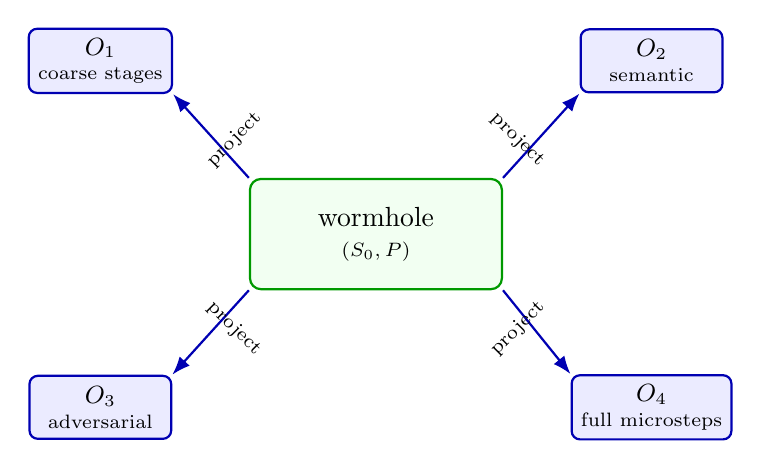
\begin{tikzpicture}[
      wormhole/.style={rectangle,draw=green!60!black,fill=green!5,thick,rounded corners,
                       minimum width=32mm,minimum height=14mm,align=center},
      observer/.style={rectangle,draw=blue!70!black,fill=blue!8,thick,rounded corners=3pt,
                       minimum width=18mm,minimum height=8mm,align=center,font=\small},
      arrow/.style={-Latex,thick},
      >=Latex
    ]

    % Central wormhole
    \node[wormhole] (W) at (0,0)
      {wormhole\\[-1pt]
       \scriptsize $(S_0,P)$};

    % Observers
    \node[observer] (O1) at (-3.5,2.2) {$O_1$\\[-2pt]\scriptsize coarse stages};
    \node[observer] (O2) at (3.5,2.2) {$O_2$\\[-2pt]\scriptsize semantic};
    \node[observer] (O3) at (-3.5,-2.2) {$O_3$\\[-2pt]\scriptsize adversarial};
    \node[observer] (O4) at (3.5,-2.2) {$O_4$\\[-2pt]\scriptsize full microsteps};

    % Projections
    \draw[arrow,blue!70!black] (W.north west) -- (O1.south east);
    \draw[arrow,blue!70!black] (W.north east) -- (O2.south west);
    \draw[arrow,blue!70!black] (W.south west) -- (O3.north east);
    \draw[arrow,blue!70!black] (W.south east) -- (O4.north west);

    % Labels on arrows
    \node[rotate=45,font=\scriptsize] at (-1.8,1.2) {project};
    \node[rotate=-45,font=\scriptsize] at (1.8,1.2) {project};
    \node[rotate=-45,font=\scriptsize] at (-1.8,-1.2) {project};
    \node[rotate=45,font=\scriptsize] at (1.8,-1.2) {project};

  \end{tikzpicture}
  \caption{Multiple observers projecting the same wormhole $(S_0,P)$
  into different trace formats.  Each observer $O_i$ extracts a
  different view of the interior evolution: coarse-grained stages,
  semantic invariants, adversarial branches, or full microsteps.
  The rulial distance measures the complexity of translating
  between these views.}
  \label{fig:observer-projections}
\end{figure}
\input{sections/multiway_ruliad}
\sectionbreak
\section{Discussion and Future Work}
\label{sec:discussion}

We have defined Recursive Metagraphs, given a deterministic concurrent
DPOI semantics, proved key confluence properties, and introduced a
holographic provenance model in which the boundary of a computation
encodes its entire interior evolution.  We have also outlined an
MDL-based rulial geometry on observers and connected RMG rewriting to
multiway systems.

\subsection{Related work}

Our work builds on several research traditions:

\paragraph{Algebraic graph rewriting.}
The DPO (Double Pushout) approach to graph rewriting was introduced
by Ehrig and others~\cite{EhrigLowe1997,EEPT06} and extended to
adhesive categories by Lack and Soboci{\'n}ski~\cite{LS06}.  We build
directly on these foundations, applying DPO semantics both to the
skeleton plane and to attachment fibers.  The tick-level confluence
theorem (\cref{thm:tick-confluence}) is a specialization of the
standard concurrency theorem for adhesive systems.

Category-theoretic graph rewriting has also been applied to
discretised space--time models in
Arrighi--Costes--Maignan~\cite{Arrighi2025Reversible}, which uses DPO
rewriting in an adhesive setting to obtain space--time deterministic
and reversible graph dynamics.  Our use of the same machinery is
conceptually similar, but we focus on deterministic multiway semantics
and holographic provenance in a computational setting rather than on
physical geometry.

\paragraph{Confluence and termination.}
The critical-pair lemma and Newman's lemma are classical tools in
term rewriting; for decreasing-diagram techniques, see van
Oostrom~\cite{vanOostrom1994}.  Our conditional global confluence
result (\cref{thm:global}) invokes these standard methods in
the graph-rewriting setting.

\paragraph{Multiway systems and the Ruliad.}
Wolfram~\cite{Wolfram2020} introduced multiway systems and the
Ruliad as a framework for fundamental physics and metamathematics.
Our RMG rewriting naturally induces multiway graphs; the determinism
discipline we impose selects unique worldlines within this larger
possibility space.  The rulial distance in Section~\ref{sec:rulial}
is our contribution to the problem of quantifying observer
differences.

\paragraph{Minimum Description Length.}
The MDL principle, pioneered by Rissanen~\cite{Rissanen1978}, provides
a rigorous information-theoretic basis for model selection and
compression.  We apply MDL to measure the complexity of
observer-to-observer translators, yielding a computable
quasi-pseudometric on the space of descriptions.

\paragraph{Categorical computation and diagrammatic reasoning.}
String diagrams and categorical algebra have been successfully applied
to quantum computing and concurrency~\cite{CoeckeDuncan2011}.  Our
two-plane fibration view (\cref{sec:determinism}) is in this
spirit: attachments live in fibers, and reindexing functors transport
attachment updates along skeleton morphisms.

The novelty of our approach lies not in any single component, but in
the synthesis: combining DPO rewriting on recursive structures,
deterministic concurrency via a two-plane discipline, and holographic
provenance encoding, all within a single framework with explicit
confluence guarantees.

Several directions remain:

\begin{itemize}[leftmargin=*]
  \item \textbf{Full global confluence analysis.}  For concrete rule
    packs used in practice, automated critical-pair analysis and
    decreasing-diagram labellings can provide machine-checkable
    confluence certificates.
  \item \textbf{Zero-knowledge provenance.}  Because payloads identify
    substructures via opaque, content-addressed pointers, it is natural
    to layer cryptographic commitments and zero-knowledge proofs on top,
    enabling external verifiers to check correctness properties without
    learning private data.
  \item \textbf{Temporal logic and Time Cube.}  The Chronos, Kairos, and Aion
    triad suggests new modal and temporal logics for reasoning about
    linear time, branch points, and the surrounding possibility space.
  \item \textbf{\COMPUTER{} architecture.}  Building on this foundation,
    the companion paper will define the \AION{} \COMPUTER{}: a machine model
    whose basic step is a provenance-carrying RMG rewrite, supporting
    backward- and forward-traceable computation, multiverse debugging,
    and glass-box AI cognition.
\end{itemize}

The long-term vision is that computational holography becomes as
standard as content-addressing and version control are today: every
nontrivial system records not just \emph{what} happened, but a
compact, verifiable encoding of \emph{how} it happened.


\bibliographystyle{alpha}
\bibliography{references}

\end{document}
